\subsection{连续高斯链模型}
\begin{center}
龚欣
\end{center}

连续高斯链是一种用于分析和数值计算的理想链模型(Doi和Edwards),该模型可以被视为离散高斯链模型的连续极限,其中的聚合物被视为一个连续的线性弹性丝(linearly elastic filament)。如图\ref{空间曲线描述聚合物构型}所示,连续高斯链的构型由空间曲线$\br (s)$描述,表示高分子长链上某一链节的位置,其中$s\in [0,N]$,被定义为路径(contour)变量。第$s$个链节在空间中的位置记为$\br (s)$,端到端向量(end-to-end-vector)$R$可以表达为$R=\br (N)−\br (0)$。
\begin{figure}[H]
\centering
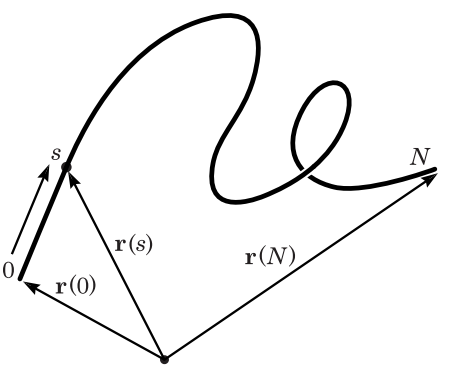
\includegraphics[scale=0.5]{./figures/41.png}
\caption{空间曲线$\br (s)$描述连续高斯链模型将聚合物的构型,其中$s\in [0,N]$是路径参数。$\br (0)$和$\br (N)$是链端位置。}
\label{空间曲线描述聚合物构型}
\end{figure}

连续高斯链的势能是
\begin{equation}
U_0[\br ]=\frac{3k_BT}{2b^2}\int_{0}^{N} \left| \frac{d\br (s)}{ds} \right|^2\mathrm{d}s \label{242}
\end{equation}
其中$U_0[\br ]$的方括号表示$U_0$是定义聚合物构型的空间曲线$\br (s)$的泛函。泛函是连续函数到数之间的映射(Volterra,1949),在上式中,这个映射是$\br (s)$与$U_0$值的关系。势能的形式与离散高斯链的方程$U_0(\bb ^N)=\sum_{i=1}^{N}h(\left|\bb _i\right|)$和$h(x)=\frac{3k_BT}{2b^2}x^2$密切相关。如果我们将$\frac{d\br (s)}{ds}$看作是高分子长链上第$s$节(链节长度为$ds$)的拉伸形变,则方程(\ref{242})是对链的整个路径上每一个这样的微分段的谐波势贡献(harmonic potential contribution)求和。值得注意的是,在连续高斯链模型中,$s$并不表示弧长,而只是表示链上各段的参数指标。因此,拉伸$\frac{d\br (s)}{ds}$不是固定的单位向量,它的大小是可以自由波动的。势能方程(\ref{242})通常称为“Edwards Hamiltonian”。

连续高斯链的构型配分函数是
\begin{equation}
Z_0=\int ~\exp(-\beta U_0[\br ])\calD \br  \label{243}
\end{equation}
其中$\int \calD \br $表示所有可能的描述聚合物的构型的空间曲线$\br (s)$上的泛函积分。这类泛函积分,又称路径积分,是量子力学和概率论领域(Feynman和Hibbs,1965)所熟悉的,其中$\br (s)$对应于量子粒子或布朗(Brownian)粒子在时间$s$时的位置。实际上,方程(\ref{243})在经典扩散(brownian motion)的路径积分中称为维纳测度(Wiener measure)。

路径积分是一种复杂的数学对象,在定义和操作上需要一定的精确性(Simon,1979)。然而在这里,我们将非正式地和以物理的方式来研究这些对象。定义路径积分有两种方法,其中一种方法是用$N_s+1$个等距路径点去离散路径,因此我们用$N_s+1$个点的空间位置逼近连续函数$\br (s)$,其中这$N_s+1$个点由向量$(\br _0,\br _1,...,\br _{N_s})$表示。这样,路径积分可以定义为$3(N_s+1)$维的普通积分(假设聚合物在体积为$V$的三维空间中)
\begin{equation}\label{244}
\int \calD \br \approx \prod_{i=0}^{N_s} \int \, \mathrm{d} \br _i
\end{equation}
其中,近似的质量随着$N_s$的增加而提高。当$N_s$有限时,连续高斯链的路径积分近似于有$N_s+1$个珠子的离散高斯链的配分函数。特别是,我们有一个近似
\begin{equation}\label{245}
Z_0=\lim_{N_s \to \infty} \prod_{j=0}^{N_s} \int \,\exp \left( -\frac{3}{2b^2\Delta s}\sum_{i=1}^{N_s}\left|\br _{i-1}-\br _i \right|^2 \right) \mathrm{d} \br _j 
\end{equation}
证明:
\begin{equation*}
\begin{aligned}
Z_0 &=\lim_{N_s \to \infty} \prod_{j=0}^{N_s} \int \,\exp\left(-\frac{3}{2b^2} \sum_{i=1}^{N_s} \int _{N_{i-1}}^{N_i} \left| \frac{\mathrm{b} \br  (s) } {\mathrm{d} s} \right|^2 \right) \mathrm{d} \br _j\\ 
& =  \lim_{N_s \to \infty} \prod_{j=0}^{N_s} \int \, \exp\left(-\frac{3}{2b^2}\sum_{i=1}^{N_s}\int _{N_{i-1}}^{N_i}\left|\frac{\br _{i-1}-\br _i}{\Delta s} \right|^2 \right)\mathrm{d} \br _j \\ 
&=  \lim_{N_s \to \infty} \prod_{j=0}^{N_s} \int \,~\exp \left( -\frac{3}{2b^2\Delta s}\sum_{i=1}^{N_s}\left|\br _{i-1}-\br _i \right|^2 \right) \mathrm{d} \br _j\\ 
\end{aligned}
\end{equation*}
其中一个$N_s$键的均方长度(mean-squared)由$b^2\Delta s$给出,$\Delta s=N/N_s$是路径点之间的间距。

方程(\ref{245})的巧妙之处源于连续极限,因为$Z_0$大小为$VN_s^{−(3/2)N_s}$,当$N_s\rightarrow \infty$时为零。通常我们对平均值感兴趣,它可以表示成两路径积分的比率。例如,连续高斯链的端到端向量的平方可以表示为
\begin{equation}\label{246}
R^2\equiv \left \langle \br \cdot \br \right \rangle _0=\frac{\int \left| \br (N)-\br (0) \right|^2~\exp(-\beta U_0[\br ]) \calD \br }{\int ~\exp(-\beta U_0[\br ]) \calD \br } 
\end{equation}
其中分母只是配分函数$Z_0$。当根据方程(\ref{246})对上述方程的分子和分母中的路径积分进行离散时,
发现奇异因子完全抵消,从而当$N_s\rightarrow \infty$时,$R^2$更好定义。此外,在路径积分的数值计算中,通常采用有限的$N_s$来避免奇异性。在整本书中,像方程(\ref{243})这样的表达式将以一种正式的方式被写和操作。我们应该意识到,在定义和估计这些对象时,可能确实存在一些微妙之处。

定义路径积分的另一种方法是通过路径的谱表示(spectral represention)。特别是,我们可以用扩充的一组完整的基函数$\lbrace \phi _0(s),\phi _1(s),... \rbrace$来表示空间曲线$\br (s)$
\begin{equation}\label{247}
\br (s)=\sum_{p=0}^{\infty} \ba _p \phi _p(s)
\end{equation}
这是一种广义的傅里叶展开式,其展开式系数$\ba _p$可以看作是广义傅里叶系数(见附录A)。对于在流体介质中自由悬浮(freely suspended in a fluid medium)的聚合物,基函数的一种方便的选择是符合“无拉伸”(no-stretch)边界条件的余弦集$\frac{d\br (s)}{ds}\vert _{s=0}=\frac{d\br (s)}{ds}\vert _{s=N}=0$。这相当于余弦傅里叶级数表示
\begin{equation}\label{248}
\br (s)=\ba _0+2\sum_{p=1}^{\infty} \ba _p \cos(p\pi s/N)
\end{equation}
根据这些基函数的正交性可以求解傅里叶系数
\begin{equation}\label{249}
\ba _p=\frac{1}{N}\int_{0}^{N} ~\cos(p\pi s/N)\br (s) \mathrm{d}s,p=0,1,2,...,\infty
\end{equation}
这些模型在聚合物文献中被称为Rouse模型,在聚合物动力学理论中起着特别重要的作用(Doi和Edwards,1986)。实际上,$\ba _0$可以解释为聚合物质心的位置,而$\ba _p,p=1,2,3,...$,尺度越细则提供更多关于聚合物形状的信息。

利用Rouse谱表示,聚合物的所有构型(路径)上的积分可以解释为对所有Rouse模型的积分的乘积。
\begin{equation}\label{250}
\int \calD \br = \prod_{p=0}^{\infty} \int \, \mathrm{d} \ba _p
\end{equation}
上述表达式右手边的对象是一个无穷维积分,所以我们再次遇到了配分函数$Z_0$的存在性问题。然而,这两个路径积分的比率是有限的,
为了数值计算的目的,我们取有限$P\gg1$使路径积分正则化(消除奇异点)
\begin{equation}\label{251}
\int \calD \br \approx \prod_{p=0}^{P} \int \, \mathrm{d} \ba _p\end{equation}
为了说明Rouse模型在连续高斯链计算中的应用,用Rouse模型表示端到端向量的平方值是
\begin{equation}\label{252}
\left | \br (N)-\br (0) \right |^2=16\sum_{p=1,3,...}^{\infty}\sum_{q=1,3,...}^{\infty} \ba _p \cdot \ba _q
\end{equation}
证明:
\begin{equation*}
\begin{aligned}
\left | \br (N)-\br (0) \right |^2 & =\left | 2\sum_{1}^{\infty}\ba _p\cos (p\pi)-2\sum_{1}^{\infty}\ba _p \right |^2\\ & =4\left | \sum_{1}^{\infty}\ba _p(\cos(p\pi)-1) \right |^2 \\ & =16\sum_{p=1,3,...}^{\infty}\sum_{q=1,3,...}^{\infty} \ba _p \cdot \ba _q\\
\end{aligned}
\end{equation*}
这个数的均值可以写为
\begin{equation}\label{253}
\left \langle \left| \br  \right|^2 \right \rangle _0=16\sum_{p=1,3,...}^{\infty}\sum_{q=1,3,...}^{\infty} \left \langle \ba _p \cdot \ba _q \right \rangle _0 
\end{equation}
其中,在Rouse模型中定义对象$f(\ba )$的均值为
\begin{equation}\label{254}
\left \langle f(\ba ) \right \rangle _0=\frac{\begin{matrix} \prod_{p=1}^{\infty} \int \,f(\ba )\exp(-\beta U_0(\ba )) \mathrm{d} \ba _p  \end{matrix}}{\begin{matrix} \prod_{p=1}^{\infty} \int \,\exp(-\beta U_0(\ba )) \mathrm{d} \ba _p  \end{matrix}}
\end{equation}
在Rouse模型表达式中,方程(\ref{242})的势能是对角的
\begin{equation}\label{255}
\beta U_0(\ba )=\frac{1}{2}\sum_{p=1}^{\infty}\alpha (p)\ba _p \cdot \ba _p
\end{equation}
其中$\alpha (p)=6\pi ^2p^2/(b^2N)$。注意,质心$p=0$模型是均匀分布。$p>0$模型都是统计独立的,是高斯分布,因此如下有(附录$B$)
\begin{equation}\label{256}
\left \langle \ba _p \cdot \ba _q \right \rangle _0=\frac{3}{\alpha (p)}\delta _{pq}
\end{equation}
替换到方程(\ref{246})将得
\begin{equation}\label{257}
\left \langle \left| \br  \right|^2 \right \rangle _0=\frac{8b^2N}{\pi ^2}\sum_{p=1,3,...}^{\infty}\frac{1}{p^2}=b^2N
\end{equation}
由此我们得出结论:连续高斯链具有离散高斯链的性质,它的端到端向量的均方值由$R=bN^{1/2}$给出。类似用期望公式给出连续高斯链的旋转半径$R_g=b(N/6)^{1/2}$。

\begin{figure}[H]
\centering
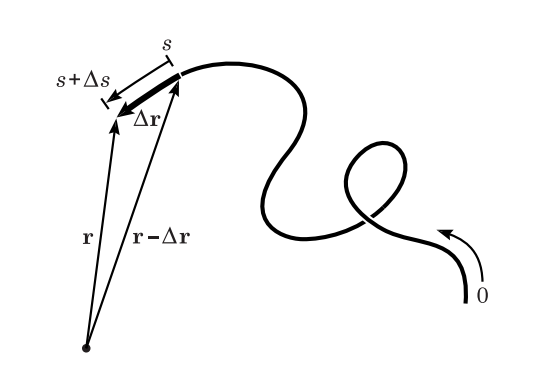
\includegraphics[scale=0.7]{./figures/42.png}
\caption{用“随机过程”(stochastic process)方法从具有$s$段的连续高斯链的统计权重中构造出具有$s+\Delta s$段的连续高斯链末端位置的统计权重。} \label{随机过程}
\end{figure}

在探索连续高斯链模型的性质时,我们现在回到了随机过程方法。具体来说,考虑一个约化的分布函数$p_0 (\br ,s)$是很有用的,它描述了在$\br$处,一个连续的路径长度为$s$的高斯链。这个函数满足归一化条件的,即$\int \,p_0(\br ,s) \mathrm{d} \br =1$。通过对离散高斯链的方程$p_0(\br ,j)=\int \,\Phi(\bb _j;\br -\bb _j)p_0(\br -\bb _j,j-1) \mathrm{d} \bb _j$的类比,我们可以通过Chapman-Kolmogorov方程利用非常小的链的信息建立分布函数
\begin{equation}\label{258}
p_0(\br ,s+\Delta s)=\int \,\Phi(\Delta \br ;\br -\Delta \br )p_0(\br -\Delta \br ,s) \mathrm{d}(\Delta \br ) 
\end{equation}

图\ref{随机过程}说明了上述方程的物理内容,它依赖于连续链的最后一部分离散化。转移概率密度$\Phi(\Delta \br ;\br -\Delta \br )$描述了路径长度$\Delta s$的链段的位移为$\Delta \br $的条件概率,从路径位置$s$处的$\br -\Delta \br $开始。连续高斯链的相关随机过程是稳定的,所以$\Phi =\Phi(\Delta \br )$与起始位置和路径位置无关。$\Phi(\Delta \br )$的表达式直接来自于连续高斯链方程(\ref{245})之前的离散化:
\begin{equation}\label{259}
\Phi(\Delta \br )=\left( \frac{3}{2\pi b^2 \Delta s} \right)^{3/2}\exp \left(- \frac{3\left| \Delta \br  \right|^2}{2b^2 \Delta s} \right) 
\end{equation}
连续链模型的一个有用的特点是,Chapman-Kolmogorov积分方程可以归结为偏微分方程,在概率论中可归结为Fokker-Planck方程(van Kampenn,1981)和量子理论中的Feynman-Kac公式(Feynman和Hibbs,1965)。我们通过导出与方程(\ref{258})相结合的Fokker-Planck方程来说明这一点。这一推导是方程的两边通过泰勒展开。注意到在这种情况下,$\Phi(\Delta \br ;\br -\Delta \br )$与初始位置$\br -\Delta \br $无关,我们不扩展转移概率。有
\begin{equation}\label{260}
\begin{aligned}
p_0(\br ,s)+\Delta s\frac{\partial}{\partial s}p_0(\br ,s)+O(\Delta s^2)=&p_0(\br ,s)-\left \langle \Delta \br  \right \rangle _\Phi \cdot \nabla p_0 (\br ,s)\\ &+\frac{1}{2!}\left \langle \Delta \br   \Delta \br  \right \rangle _\Phi:\nabla \nabla p_0(\br ,s)\\ &+O(\left \langle \Delta \br   \Delta \br   \Delta \br  \right \rangle _\Phi)
\end{aligned}
\end{equation}
其中,该方程中出现的$\Phi$平均定义为
\begin{equation}\label{261}
\left \langle f(\Delta \br ) \right \rangle _\Phi = \int \,\Phi (\Delta \br )f(\Delta \br ) \mathrm{d}(\Delta \br )
\end{equation}
利用方程(\ref{259})的显式高斯形式,可以将方程(\ref{260})右侧的平均值计算为(附录$B$)
\begin{equation}\label{262}
\left \langle \Delta \br  \right \rangle _\Phi = 0
\end{equation}
\begin{equation}\label{263}
\left \langle \Delta \br _\alpha \Delta \br _\beta \right \rangle _\Phi = \frac{b^2 \Delta s}{3}\delta_{\alpha \beta}
\end{equation}
如果我们将这些式子带入方程(\ref{260})中,则$\Delta s \rightarrow \infty$时的分布函数$p_0(\br ,s)$满足Fokker-Planck方程

\begin{equation}\label{264}
\frac{\partial}{\partial s}p_0(\br ,s)=\frac{b^2}{6}\nabla ^2 p_0(\br ,s) 
\end{equation}

因此,连续高斯链的Fokker-Planck方程给出的具有“扩散系数”$b^2/6$
的传统扩散方程的形式。该方程的解提供了关于端点段$p_0(\br ,s)$分布的完整信息。

Fokker-Planck方程是特别方便,因为有各种各样的分析和数值技术可用于求解偏微分方程。对于方程(\ref{264}),对应于初始条件$p_0(\br ,s)=\delta(\br )$的基本(格林函数)解是
\begin{equation}\label{265}
p_0(\br ,s)=\left[ 3/(2 \pi sb^2) \right]^{3/2}\exp \left[ -3\left| \br  \right|^2/(2sb^2) \right]
\end{equation}
如果令$s=N,\br =\br $,则端到端向量恢复成熟悉的高斯分布函数(\ref{243})
在比单键更大的尺度下,离散高斯链和连续高斯链明显具有相同的链端分布函数。使用连续链的优点是它允许用偏微分方程进行计算。这一优势将在第三章中变得更加明显,在第三章中,我们将考虑有外势的链。
\endinput